% The direction and separation network for one 128 ms chunk (T = 8 frames), read left to right.
% From ros2_ws/src/doa_separation_node/doa_separation_node/model/net_v3.py and mamba_block.py; sizes are in the README table.
% Grids: the slice of the bins x time plane each block works on. Orange: state kept from one chunk to the next.
\documentclass[border=1.5pt]{standalone}
% Shared look of the figures in docs/. Text 8 pt, Times.
% Colors: cInk for this device's code and data, cFace (grey fill) for hardware, cCal for the one point each figure is about.
\usepackage[T1]{fontenc}
\usepackage{times}
\usepackage{amsmath,amssymb}
\usepackage{xcolor}
\usepackage{tikz}
\usepackage{pgfplots,pgfplotstable}
\pgfplotsset{compat=1.18}
\usetikzlibrary{arrows.meta,positioning,calc}
\usepgfplotslibrary{groupplots}

\definecolor{cCal}{HTML}{D55E00}
\definecolor{cInk}{HTML}{1F2933}
\definecolor{cMuted}{HTML}{6B7280}
\definecolor{cGrid}{HTML}{E3E6EA}
\color{cInk}

\newcommand{\figfont}{\fontsize{8}{9.5}\selectfont}
\newcommand{\figsmall}{\fontsize{8}{9.5}\selectfont}

\pgfplotsset{
  spl/.style={
    width=44mm, height=36mm, scale only axis=false,
    axis line style={cMuted, line width=0.5pt},
    tick style={cMuted, line width=0.5pt}, tick align=outside,
    tick label style={font=\figsmall, text=cInk},
    label style={font=\figfont, text=cInk},
    legend style={font=\figsmall, draw=none, fill=none, text=cInk, inner sep=0pt},
    legend cell align=left,
    grid=major, major grid style={cGrid, line width=0.4pt},
    axis lines*=left, clip mode=individual,
    every axis plot/.append style={line width=0.9pt},
  },
}

\begin{document}
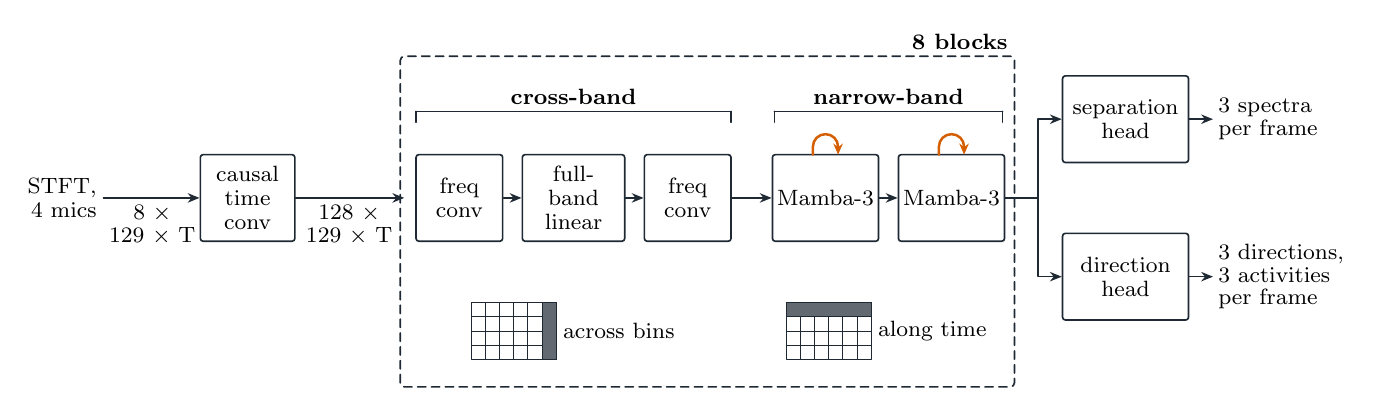
\begin{tikzpicture}[x=1mm, y=1mm, font=\figfont, line join=round, line cap=round,
  own/.style={draw=cInk, line width=0.6pt, rounded corners=1pt, align=center, inner xsep=0.6mm, inner ysep=0.8mm, fill=white, minimum height=11mm},
  flow/.style={-{Stealth[length=1.5mm, width=1.2mm]}, line width=0.6pt, draw=cInk},
  dim/.style={inner sep=0.8mm, align=center},
  loop/.style={cCal, line width=0.9pt, -{Stealth[length=1.4mm, width=1.2mm]}},
  cell/.style={draw=cInk, line width=0.3pt}]

\node[anchor=east, align=right, inner sep=0pt] at (9,30) {STFT,\\[-0.3mm]4 mics};
\draw[flow] (9.8,30) -- (22,30);
\node[dim, anchor=north] at (16,30) {8 $\times$\\[-0.4mm]129 $\times$ T};
\node[own, minimum width=12mm, anchor=west] (enc) at (22,30) {causal\\[-0.3mm]time\\[-0.3mm]conv};
\draw[flow] (enc.east) -- (48,30);
\node[dim, anchor=north] at (41,30) {128 $\times$\\[-0.4mm]129 $\times$ T};
\begin{scope}[xshift=2.5mm]

\draw[cInk, line width=0.6pt, densely dashed, rounded corners=1.5pt] (45,6) rectangle (123,48);
\node[anchor=south east, inner sep=0.8mm] at (123,48) {\textbf{8 blocks}};
\node[own, minimum width=11mm] (fc1) at (52.5,30) {freq\\[-0.3mm]conv};
\node[own, minimum width=13mm] (fb)  at (67,30) {full-\\[-0.3mm]band\\[-0.3mm]linear};
\node[own, minimum width=11mm] (fc2) at (81.5,30) {freq\\[-0.3mm]conv};
\node[own, minimum width=13mm] (m1)  at (99,30) {Mamba-3};
\node[own, minimum width=13mm] (m2)  at (115,30) {Mamba-3};
\draw[flow] (fc1.east) -- (fb.west);
\draw[flow] (fb.east) -- (fc2.west);
\draw[flow] (fc2.east) -- (m1.west);
\draw[flow] (m1.east) -- (m2.west);
\draw[cInk, line width=0.5pt] (47,41) -- (87,41) (47,41) -- (47,39.6) (87,41) -- (87,39.6);
\node[anchor=south, inner sep=0.8mm] at (67,41) {\textbf{cross-band}};
\draw[cInk, line width=0.5pt] (92.5,41) -- (121.5,41) (92.5,41) -- (92.5,39.6) (121.5,41) -- (121.5,39.6);
\node[anchor=south, inner sep=0.8mm] at (107,41) {\textbf{narrow-band}};
\foreach \cx in {99,115} {
  \draw[loop] (\cx-1.6,35.5) -- ++(0,1.0) arc[start angle=180, end angle=0, radius=1.6] -- ++(0,-1.0); }

\foreach \i in {0,...,5} { \foreach \j in {0,...,3} {
  \draw[cell] (54.0+1.8*\i,9.5+1.8*\j) rectangle ++(1.8,1.8);
  \draw[cell] (94.0+1.8*\i,9.5+1.8*\j) rectangle ++(1.8,1.8); } }
\fill[cInk!70] (54.0+1.8*5,9.5) rectangle ++(1.8,7.2);
\draw[cell] (54.0+1.8*5,9.5) rectangle ++(1.8,7.2);
\fill[cInk!70] (94.0,9.5+1.8*3) rectangle ++(10.8,1.8);
\draw[cell] (94.0,9.5+1.8*3) rectangle ++(10.8,1.8);
\node[anchor=west, inner sep=0pt] at (65.6,13.1) {across bins};
\node[anchor=west, inner sep=0pt] at (105.6,13.1) {along time};

\draw[line width=0.6pt, draw=cInk] (m2.east) -- (126,30);
\draw[flow] (126,30) |- (129,40);
\draw[flow] (126,30) |- (129,20);
\node[own, anchor=west, minimum width=16mm] (sep) at (129,40) {separation\\[-0.3mm]head};
\node[own, anchor=west, minimum width=16mm] (doa) at (129,20) {direction\\[-0.3mm]head};
\draw[flow] (sep.east) -- ++(3,0);
\draw[flow] (doa.east) -- ++(3,0);
\node[anchor=west, inner sep=0.6mm, align=left] at ($(sep.east)+(3,0)$) {3 spectra\\[-0.5mm]per frame};
\node[anchor=west, inner sep=0.6mm, align=left] at ($(doa.east)+(3,0)$) {3 directions,\\[-0.5mm]3 activities\\[-0.5mm]per frame};
\end{scope}
\end{tikzpicture}
\end{document}
